\documentclass[hyperref]{beamer}
\usepackage{beamerthemesplit}
\usepackage{graphicx}
\usepackage{mathptmx}           % replacement for obsolete \usepackage{times}
\usepackage[scaled=1.0]{helvet} % replacement for obsolete \usepackage{times}
\usepackage{courier}            % replacement for obsolete \usepackage{times}
\usepackage[normalem]{ulem}

\usepackage{tikz}
\usetikzlibrary{shapes.arrows,chains,positioning,automata,trees,calc}
\usetikzlibrary{patterns}
\usetikzlibrary{decorations.pathmorphing,decorations.markings}
\usepackage{times,latexsym,amsfonts,amssymb,amsmath,graphicx,url,bbm,rotating,siunitx}
\usepackage{multirow,hhline,arydshln,array,color,stmaryrd,pifont,transparent}
\usepackage[absolute,overlay]{textpos}
\definecolor{darkred}{rgb}{0.5, 0.0, 0.0}
\definecolor{darkgreen}{rgb}{0.0, 0.4, 0.0}
\definecolor{darkblue}{rgb}{0.0, 0.0, 0.5}

% set up Beamer style with Stanford colors and logo
% logo is available at http://nlp.stanford.edu/local/nlp-logos/nlp-logo.pdf
\useinnertheme{rounded}
\useoutertheme{infolines}
\usecolortheme{beaver}
\setbeamercolor{block title}{fg=white,bg=darkred!75!black}
\setbeamercolor{block body}{parent=normal text,bg=black!5!bg}
\setbeamercolor{item projected}{bg=darkred}
\logo{
\includegraphics[height=1cm]{nlp-logo.pdf}}

% Macros
\def\blue#1{\textcolor{blue}{#1}}
\def\darkblue#1{\textcolor{blue}{#1}}
\def\red#1{\textcolor{red}{#1}}
\def\darkred#1{\textcolor{darkred}{#1}}
\def\green#1{\textcolor{green}{#1}}
\def\darkgreen#1{\textcolor{darkgreen}{#1}}
\def\yellow#1{\textcolor{yellow}{#1}}
\def\orange#1{\textcolor{orange}{#1}}
\def\gray#1{\textcolor{gray}{#1}}
\def\darkgray#1{\textcolor{darkgray}{#1}}
\newcommand\w[1]{\textit{\darkgreen{#1}}}
\newcommand\ww[1]{\textit{#1}}
\newcommand\h[1]{\textbf{#1}}
\newcommand\hh[1]{\textbf{\textcolor[rgb]{0.5,0,0}{#1}}}

% title page information
\title[Robust Subgraphs for AMR]{Robust Subgraph Generation for Abstract Meaning Representation
Parsing}
\subtitle{}
\author[Werling, Angeli, Manning]{Keenon Werling, \darkblue{Gabor Angeli}, Chris Manning}
\date{May 30, 2015}
\institute[Stanford]{Stanford University}


\begin{document}
\begin{frame}[noframenumbering]
  \titlepage
\end{frame}

%%%%%%%%%%%%%%%%%%%%%%%%%%%%%%%%%%%%%%%%%%%%%%%%%%%%%%%%%%%%%%%%%%%%%%%%%%%%%%%
% What is AMR?
%%%%%%%%%%%%%%%%%%%%%%%%%%%%%%%%%%%%%%%%%%%%%%%%%%%%%%%%%%%%%%%%%%%%%%%%%%%%%%%

\begin{frame}[noframenumbering]{Keenon Werling}
\begin{center}
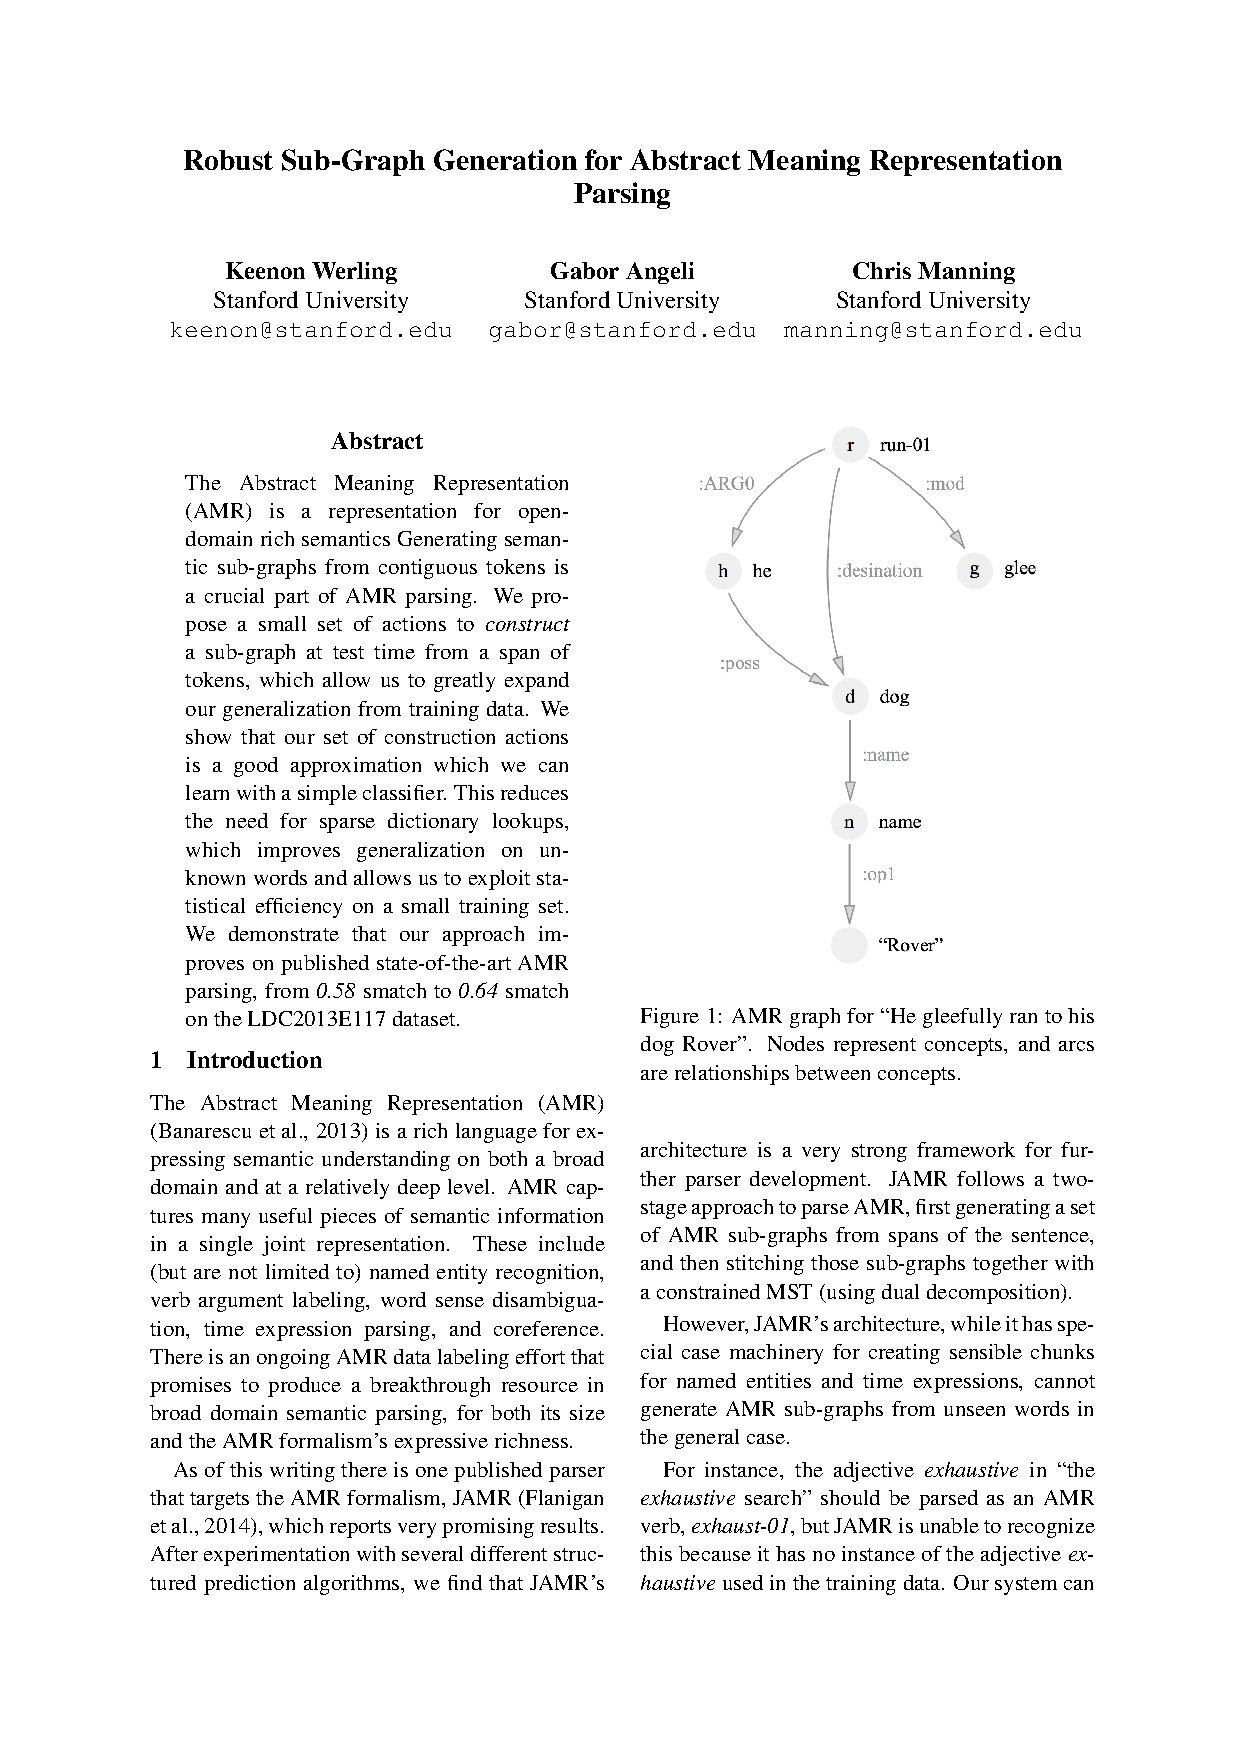
\includegraphics[scale=0.15]{keenon.jpg}
\newline
TODO A picture of Keenon
\end{center}
\end{frame}

%%%%%%%%%%%%%%%%%%% 
% Intro
%%%%%%%%%%%%%%%%%%%
\begin{frame}{What is The Abstract Meaning Representation?}
\begin{center}
\hh{A semantic representation for language as a rooted, directed graph}
\end{center}
\begin{tabular}{lcl}
\w{``He gleefully ran to his dog rover''} &
$\rightarrow$ &
\raisebox{-.5\height}{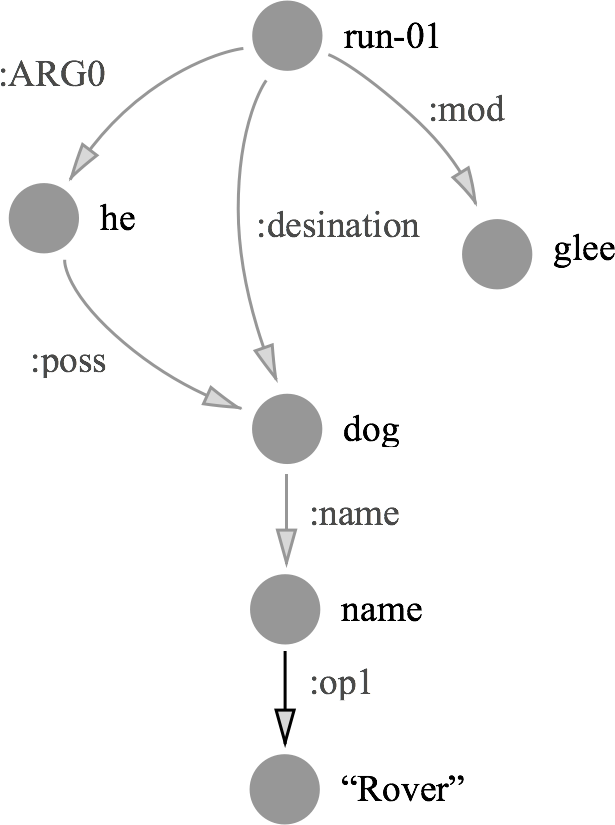
\includegraphics[scale=0.20]{glee.png}}
\end{tabular}
\end{frame}

%%%%%%%%%%%%%%%%%%% 
% Decompose AMR
%%%%%%%%%%%%%%%%%%%
\begin{frame}{Decomposing AMR}
\begin{center}
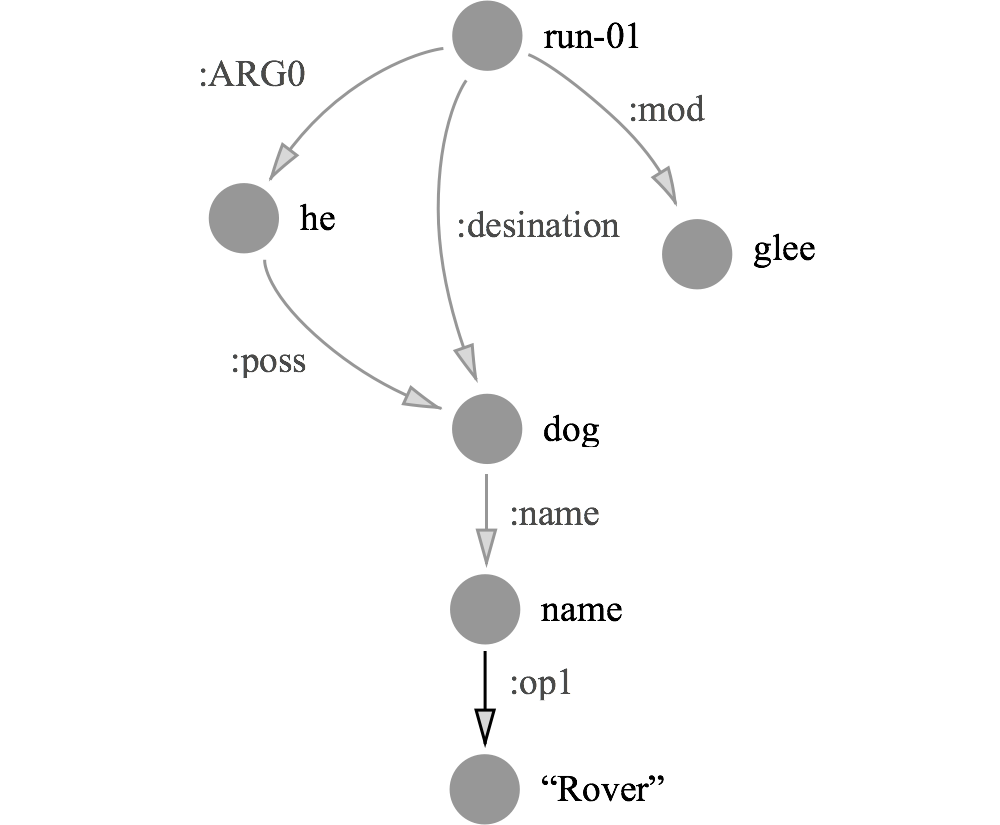
\includegraphics[scale=0.25]{glee_base.png}
\end{center}
\end{frame}

\begin{frame}[noframenumbering]{Decomposing AMR}
\begin{center}
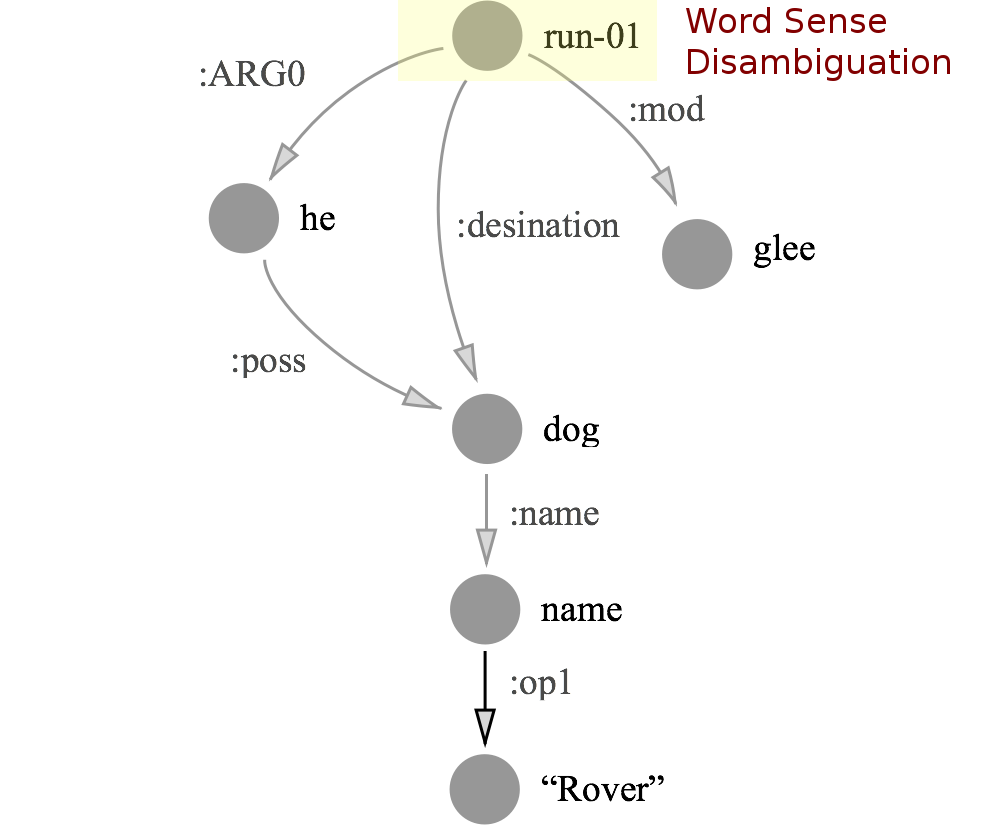
\includegraphics[scale=0.25]{glee_wsd.png}
\end{center}
\end{frame}

\begin{frame}[noframenumbering]{Decomposing AMR}
\begin{center}
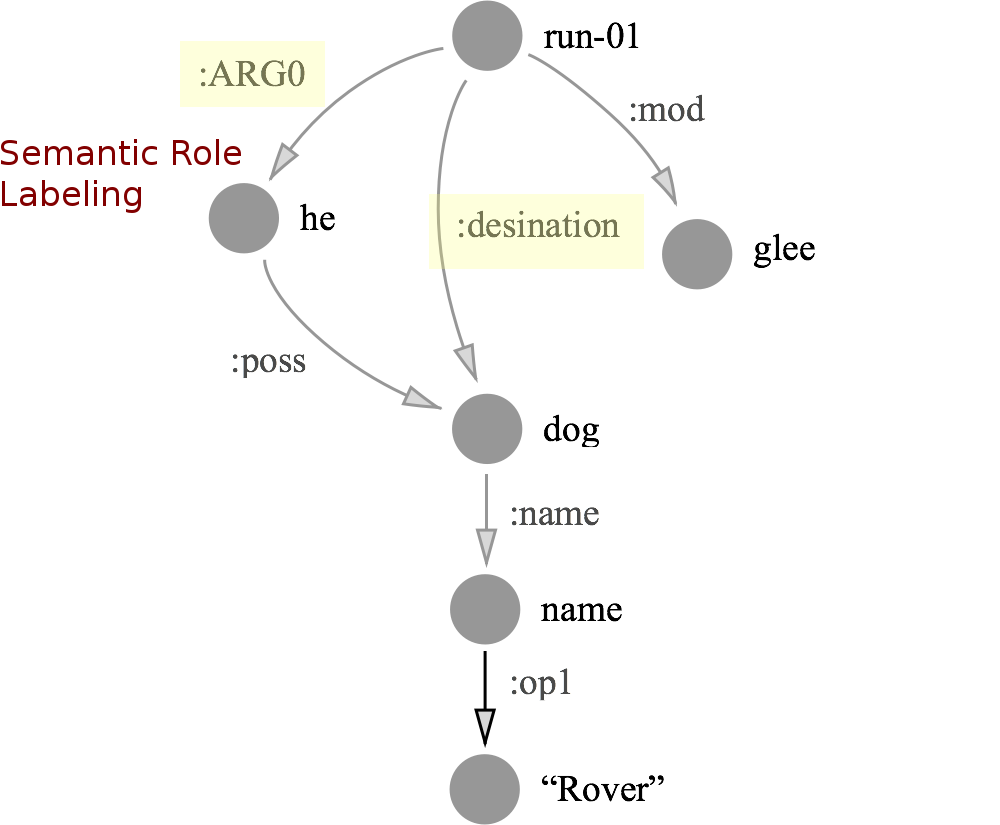
\includegraphics[scale=0.25]{glee_srl.png}
\end{center}
\end{frame}

\begin{frame}[noframenumbering]{Decomposing AMR}
\begin{center}
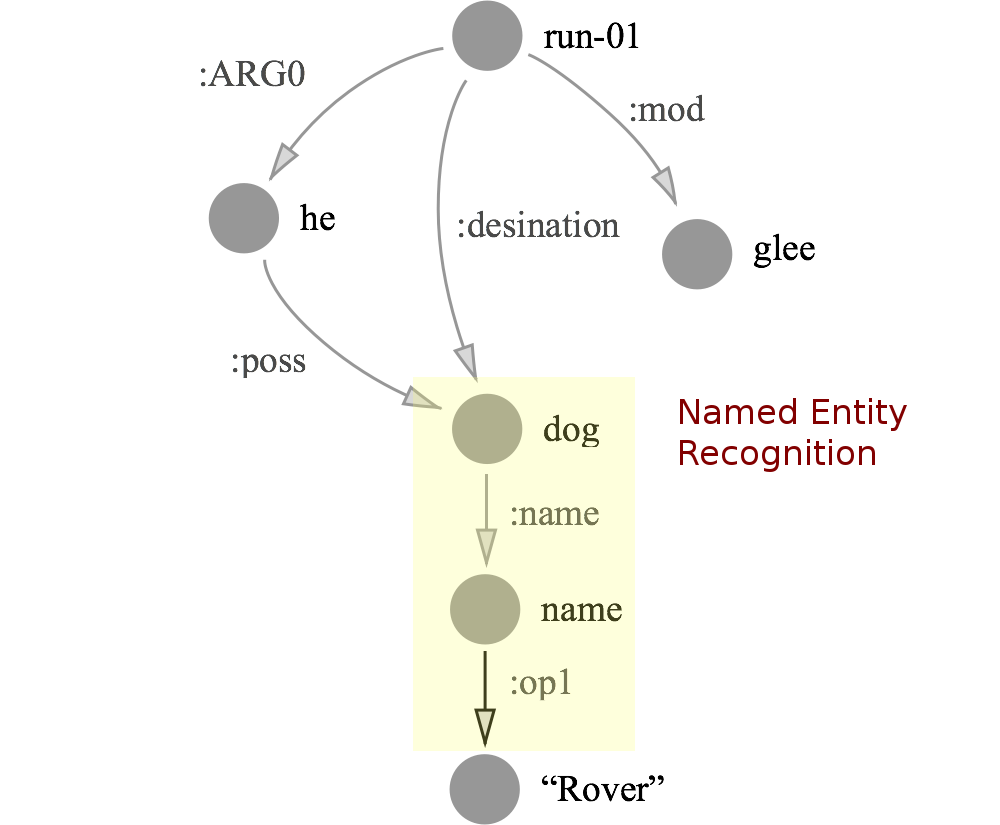
\includegraphics[scale=0.25]{glee_ner.png}
\end{center}
\end{frame}

\begin{frame}[noframenumbering]{Decomposing AMR}
\begin{center}
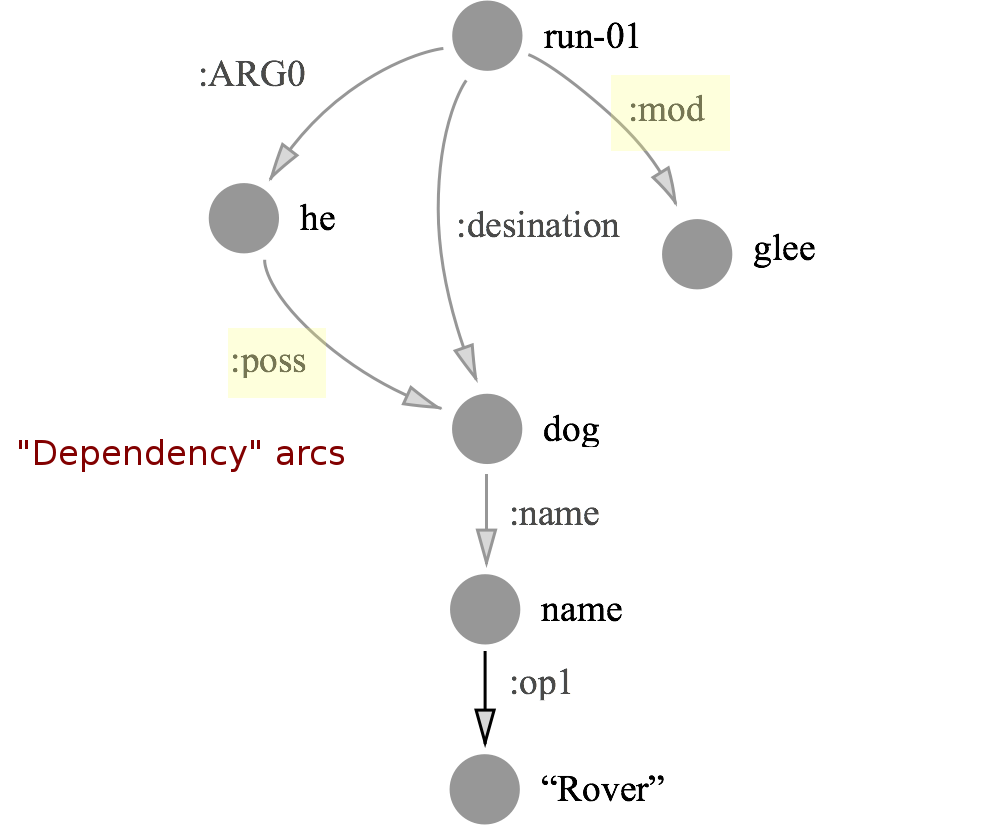
\includegraphics[scale=0.25]{glee_deps.png}
\end{center}
\end{frame}

%%%%%%%%%%%%%%%%%%% 
% NER++ and SRL++
%%%%%%%%%%%%%%%%%%%
\begin{frame}{Insight from JAMR: Two Classes of Phenomena}
\begin{center}
\begin{tabular}{cc}
``SRL++''& \raisebox{-0.5\height}{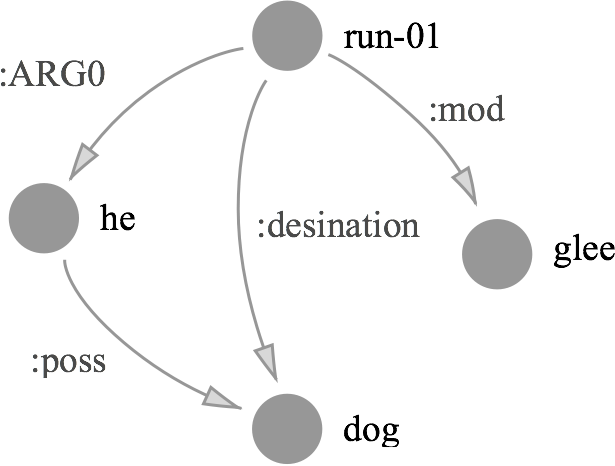
\includegraphics[scale=0.20]{srl_only.png}} \\
& \\
``NER++'' & \raisebox{-0.5\height}{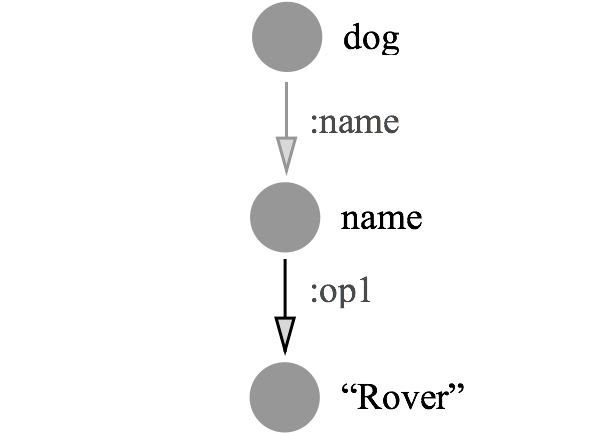
\includegraphics[scale=0.20]{ner_only.png}} \\
\end{tabular}
\end{center}
\end{frame}


%%%%%%%%%%%%%%%%%%% 
% Pipeline
%%%%%%%%%%%%%%%%%%%
\begin{frame}{Pipeline: Start with text}
\begin{center}
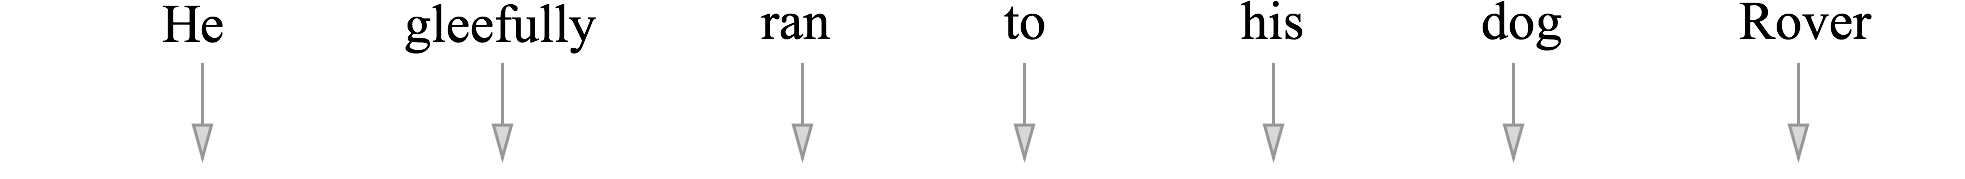
\includegraphics[scale=0.17]{concept_1.png}
\end{center}
\end{frame}

\begin{frame}[noframenumbering]{Pipeline: Generate subgraphs}
\begin{center}
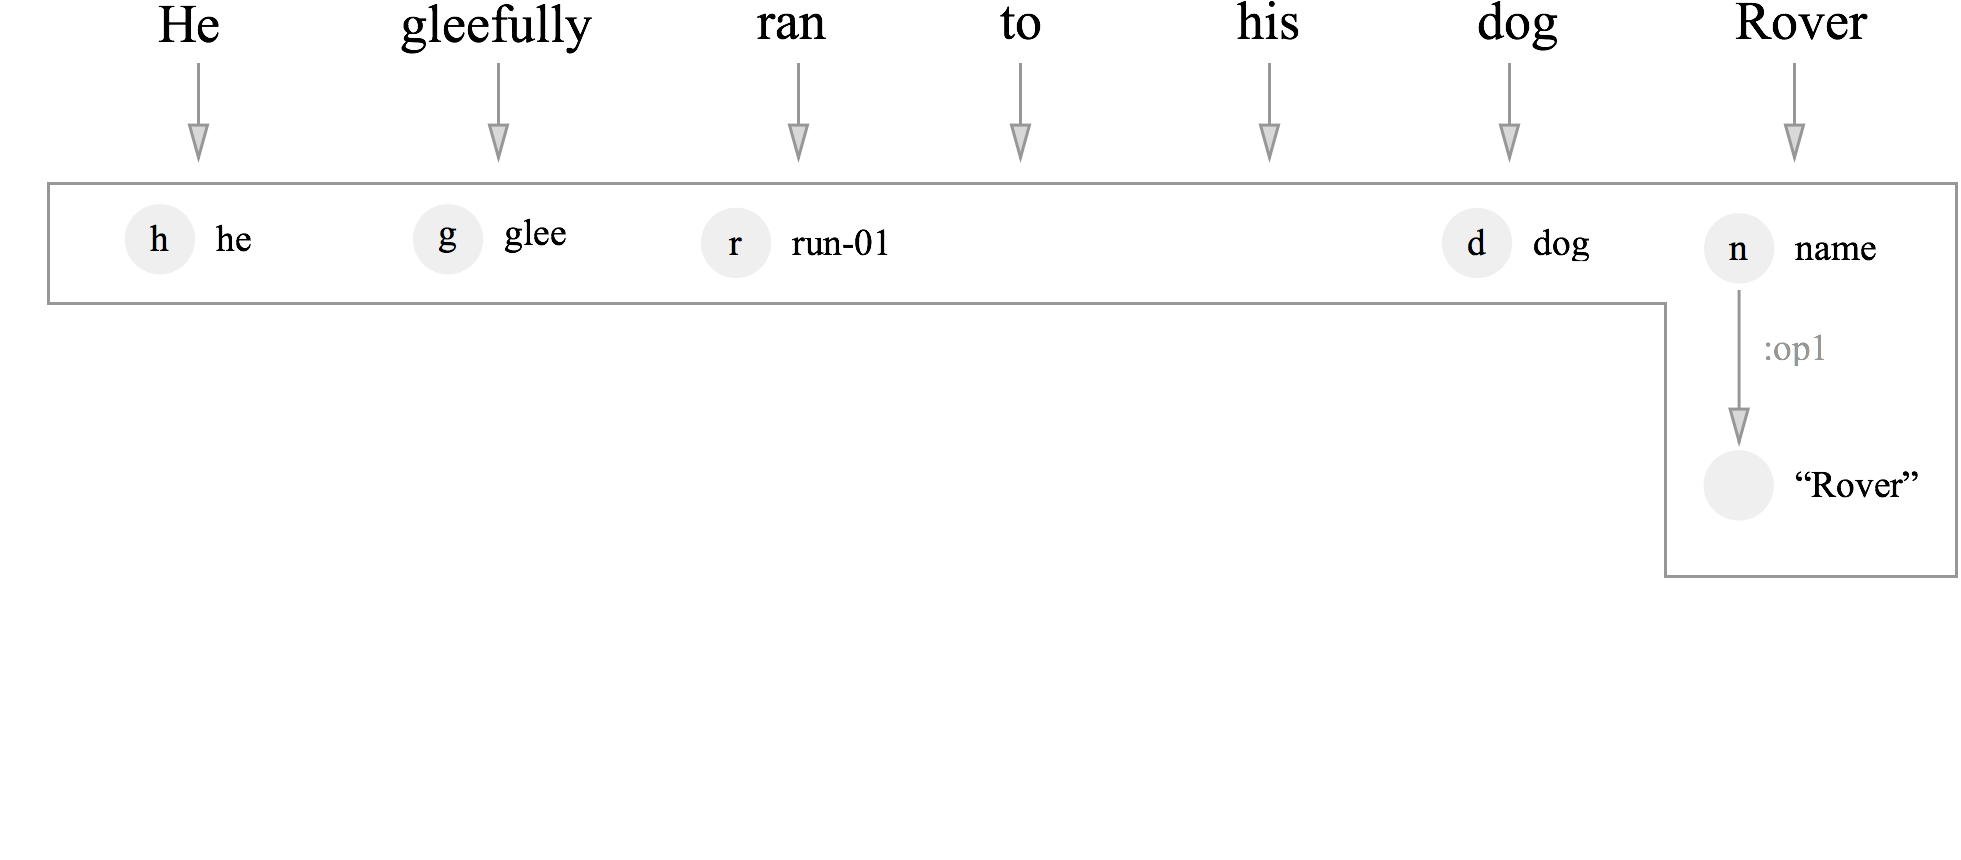
\includegraphics[scale=0.17]{concept_2.png}
\end{center}
\end{frame}

\begin{frame}[noframenumbering]{Pipeline: Link subgraphs}
\begin{center}
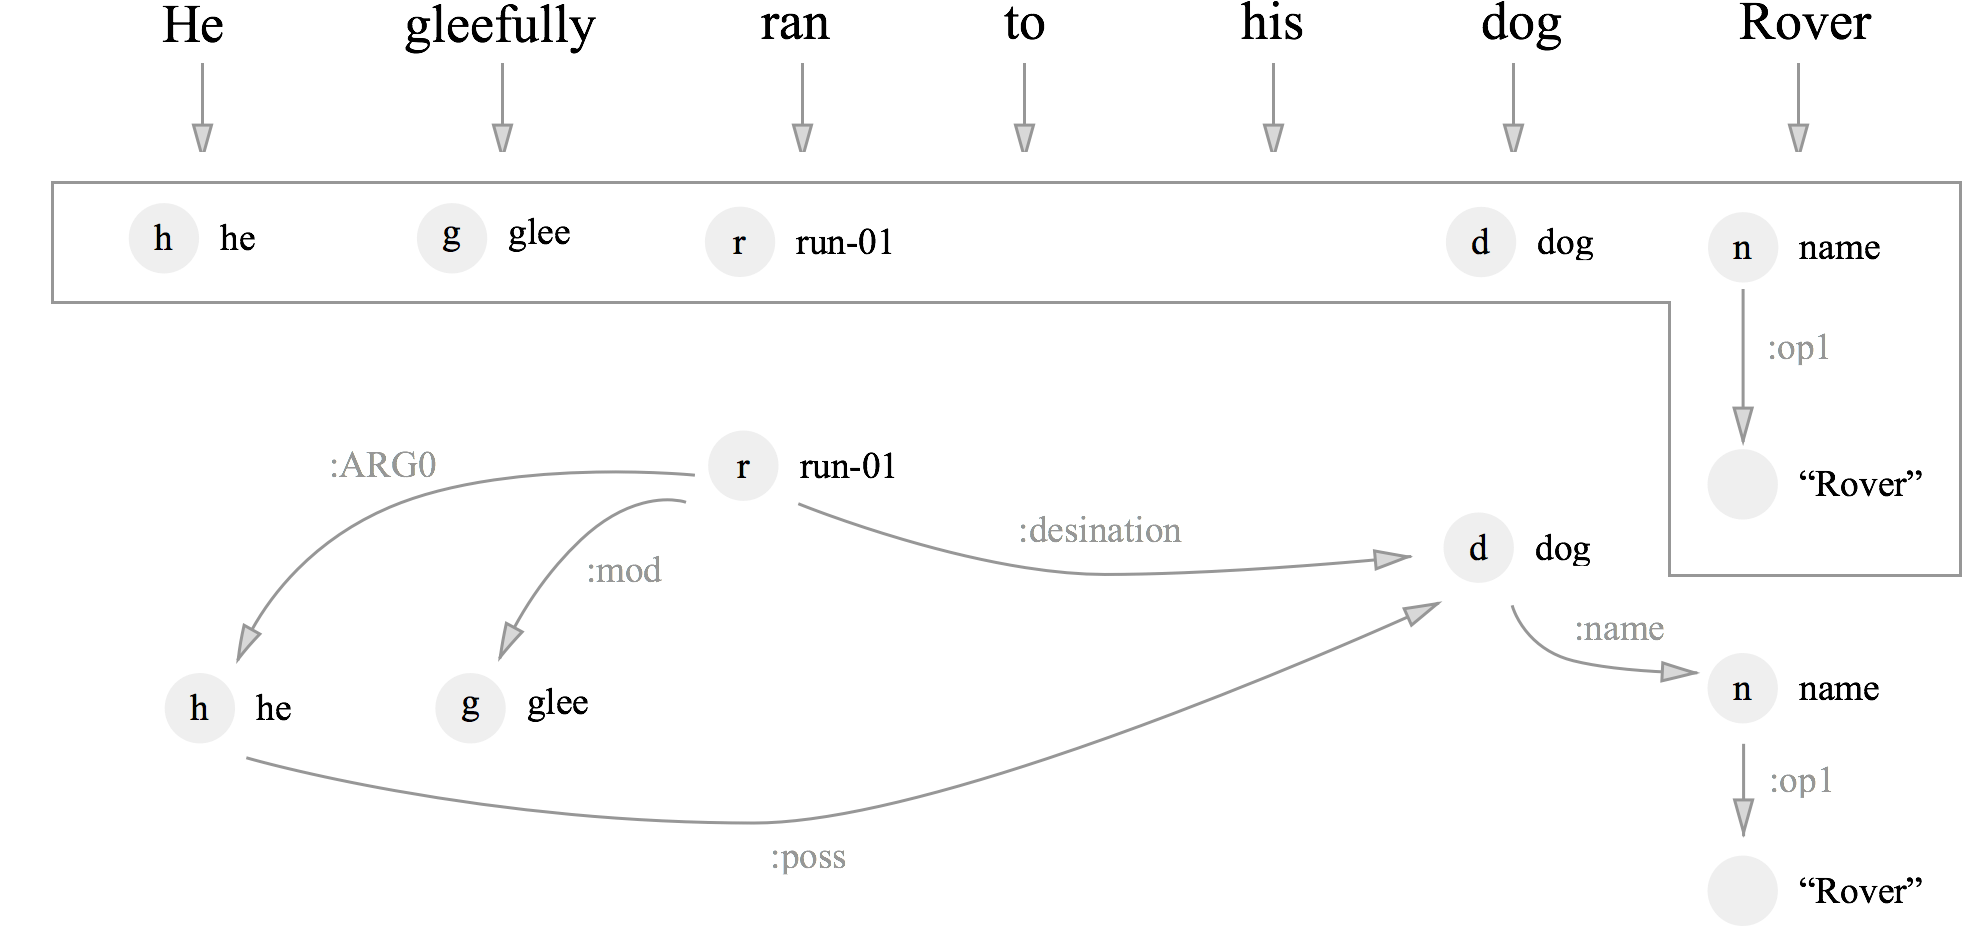
\includegraphics[scale=0.17]{concept_3.png}
\end{center}
\end{frame}


%%%%%%%%%%%%%%%%%%% 
% NER++ is hard
%%%%%%%%%%%%%%%%%%%
\begin{frame}{Observation: NER++ is Surprisingly Hard}
\begin{center}
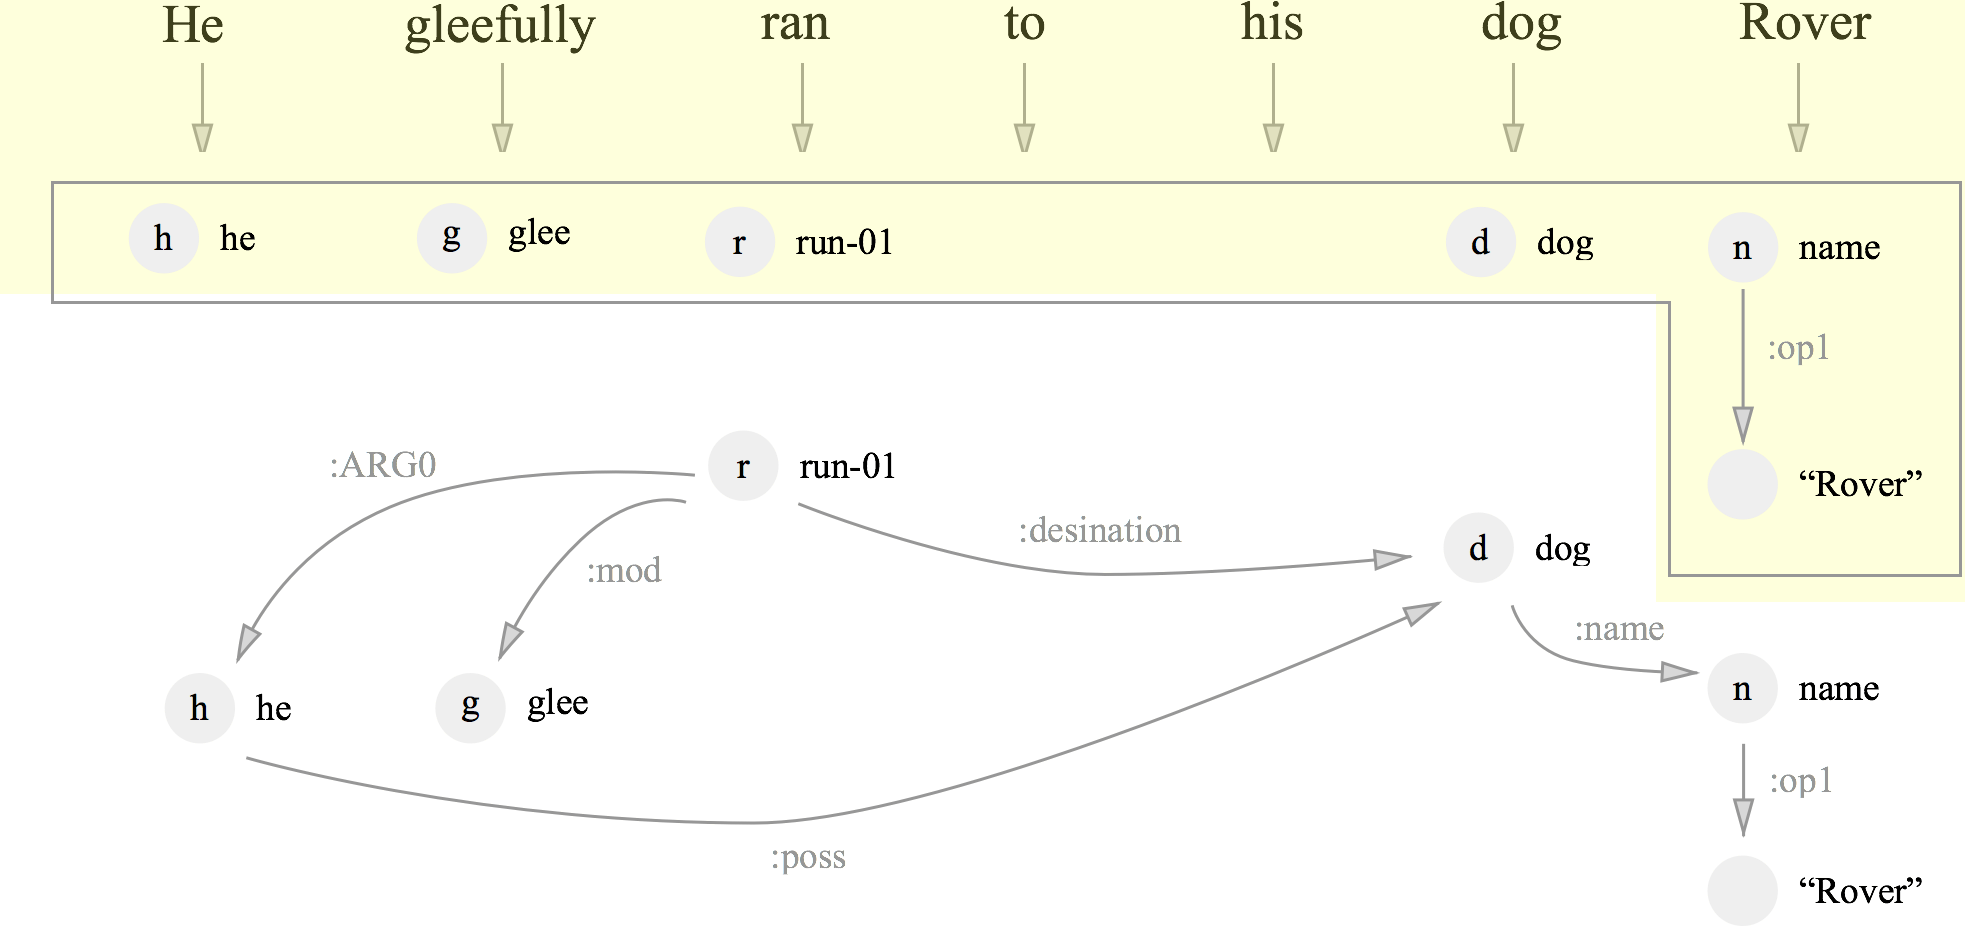
\includegraphics[scale=0.17]{concept_hard.png}
\end{center}
\end{frame}

\begin{frame}[noframenumbering]{Observation: NER++ is Surprisingly Hard}
\hh{From Flanigan et al. (2014):}

\begin{center}
\begin{tabular}{lccc}
\hline
System & Precision & Recall & F$_1$ \\
\hline
Gold NER++      & 76 & 84 & 80 \\
Predicted NER++ & 52 & 66 & 58 \\
\hline
\end{tabular}
\end{center}

\begin{itemize}
\item 22\% Performance loss on NER++
\item Even larger than the 20\% performance loss on SRL++
\end{itemize}
\end{frame}

%%%%%%%%%%%%%%%%%%% 
% Contribution: Actions
%%%%%%%%%%%%%%%%%%%
\begin{frame}{Contribution: Factor NER++ into \textit{Actions}}
\begin{center}
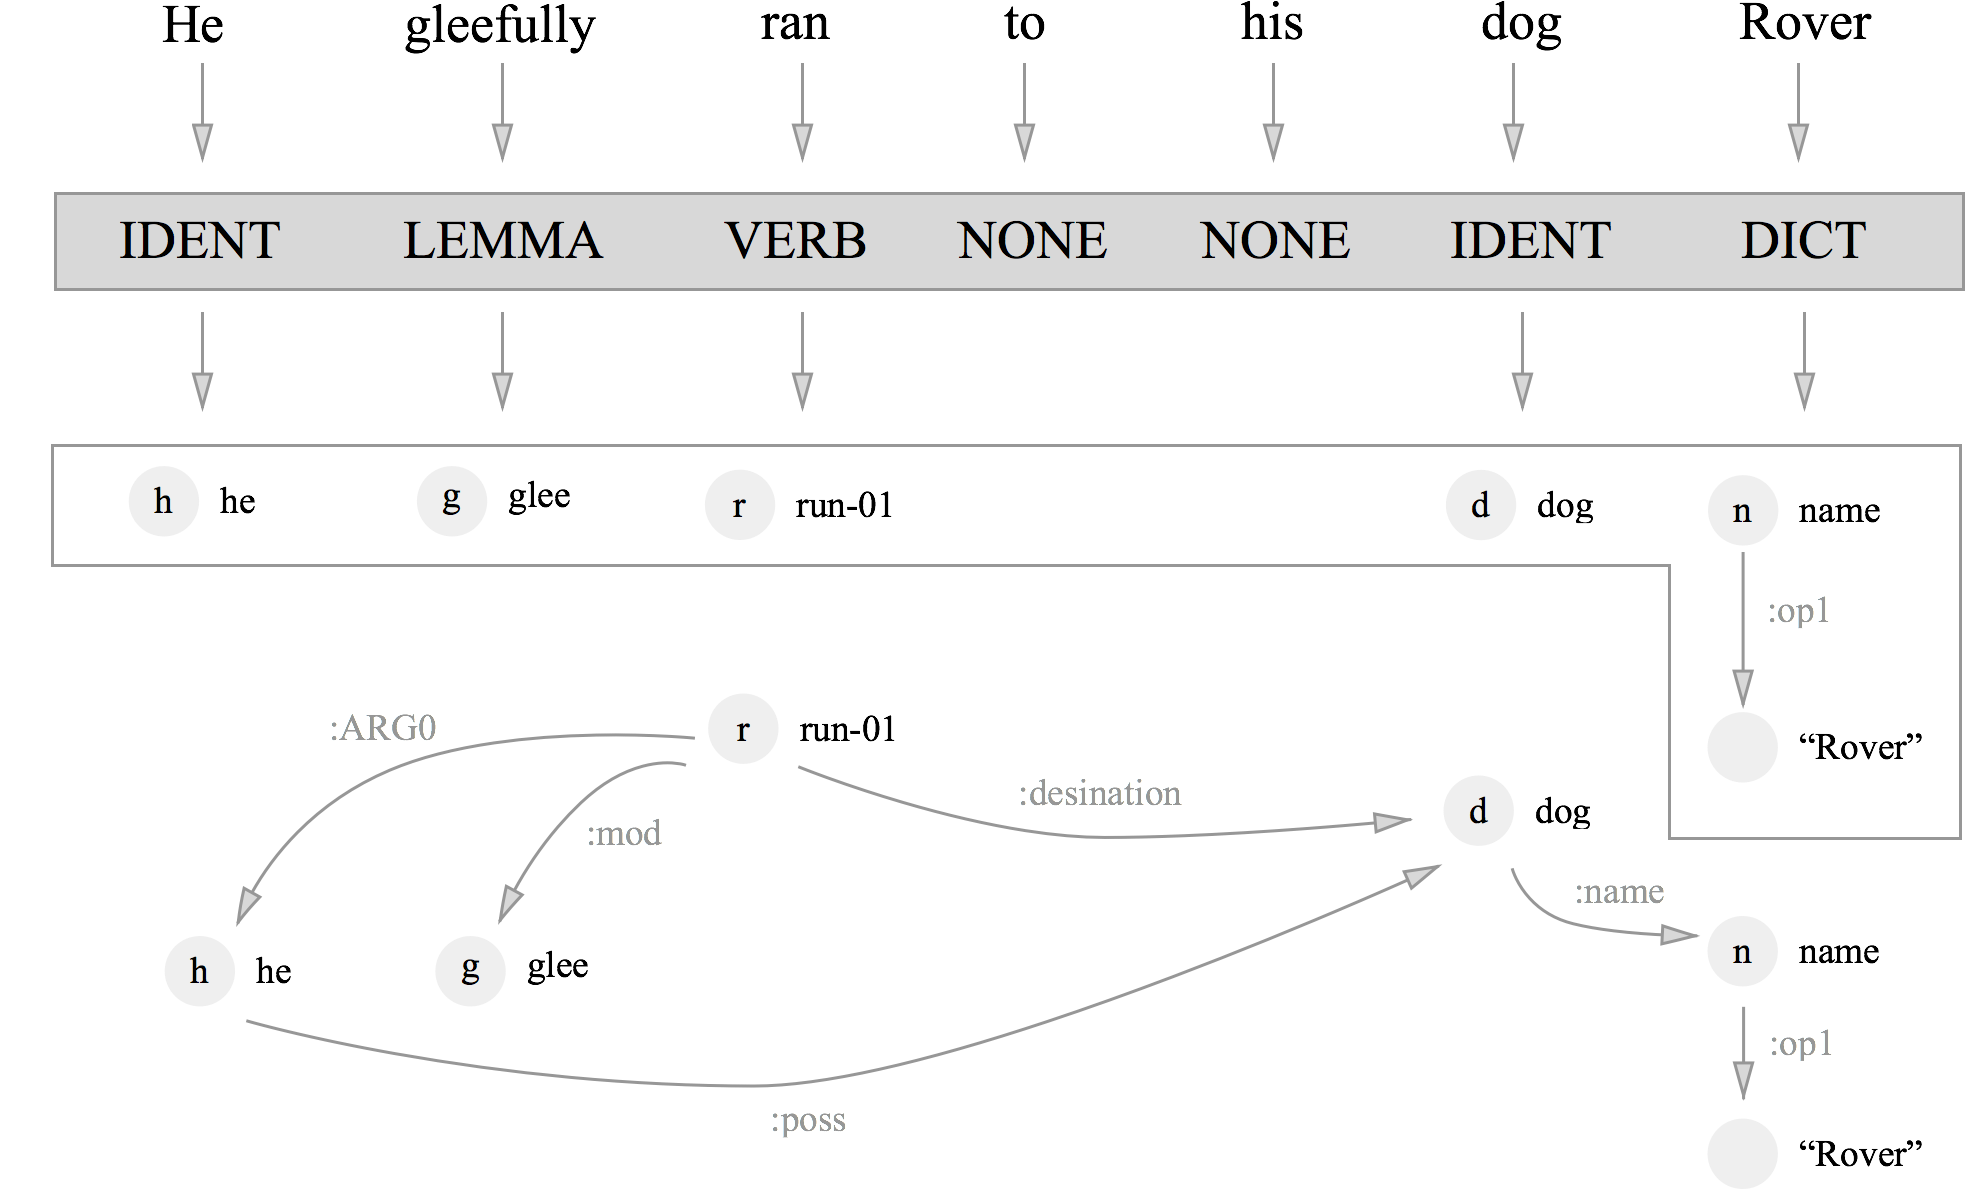
\includegraphics[scale=0.17]{concept.png}
\end{center}
\end{frame}

%%%%%%%%%%%%%%%%%%% 
% List Actions
%%%%%%%%%%%%%%%%%%%
\begin{frame}{Contribution: Factor NER++ into \textit{Actions}}

%%%%%%%%%%%%%%%%%%% 
% THANKS
%%%%%%%%%%%%%%%%%%%


\end{document}
